\documentclass[12pt,letterpaper]{ntdhw}


\usepackage{ntdmath}

\title{Project 1: Regular Languages and Pursuit-Evasion}
\author{CSCI 561}

\rhead{Names:}

%\keytrue

\begin{document}
\pagestyle{fancyplain}

\maketitle
\thispagestyle{fancyplain}
%\clearpage



\section*{Application: Text Processing with Grep}

\begin{quote}
  \emph{\texttt{grep} is a unix utility that searches text for lines
    matching a regular expression.}
\end{quote}

\begin{enumerate}
  \item \textbf{Using Grep:} Use the standard unix (or GNU)
  \texttt{grep} and the implementation in this project to search the
  starter code for all \texttt{TODO}s.
  \begin{figure}[htp]
    \centering
    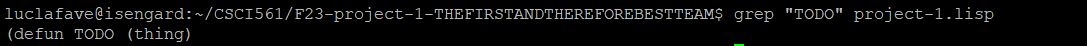
\includegraphics[width=17cm]{unixGrep.JPG}
    \caption{Unix Grep}
\end{figure}

  \item \textbf{NFA vs. DFA Simulation:} The original grep utility (as
  written by Ken Thompson) converted the provided regular expression
  to an NFA and then simulated the NFA on the input text.  Why would
  Thompson have used NFA simulation instead of DFA simulation?
  \par \textbf{Answer 2:} I would assume he made this choice for a couple of reasons. The first is I believe that Thompson in 1972 was probably memory constrained, but converting from an NFA to a DFA usually results in a larger DFA. The worst case can be up to $2^n$ nodes more in DFA than NFA  which is exponentially bad in memory constrained environments. Another reason I believe this decision was made is that on top of the memory constraint issues the time it takes to preform subset construction to convert an NFA to a DFA added plus the time to then preform dfa-simulate was usually not much faster than just preforming Thompson's implementation of  nfa-simulate, especially if most nfa's created did not end up being extremely complicated. 

  \item \textbf{Time Complexity:} To simulate an NFA
  $N=\lmtuple{Q}{\Sigma}{\delta}{q_0}{F}$ on string $\sigma$ using the
  algorithm in the original grep (which is roughly equivalent to the
  NFA simulation algorithm covered in lecture) requires
  $O(|Q|*|\sigma|)$ time. However, many ``regex'' engines (including the
  popular implementation in Perl) exhibit worst-case complexity that
  is exponential in $|\sigma|$.

  \begin{enumerate}
    \item Prove that NFA simulation is possible in $O(|Q|*|\sigma|)$
      time.%
      \par \textbf{Answer 3a:} Using Thompson's implementation of NFA simulate it is possible to preform the algoritm in the runtime of $O(|Q|*|\sigma|)$. 1. Initialize two lists a current states list and a list of next states.
    2. Fill current states list with the start state. 
    3. For each character in the string loop through the current states and find the next states add to list. If one next state is an accept state break and print string in language. 
    4. set current states list to be next states list then move to next string. If no new next states break and print string not in language.
    5. This is time complexity of $|\sigma| * |Q|$ because you go through length of string and for each character you loop through each state. The worst case can be looping through all the states in the NFA which is $|Q|$. This means that it could end up taking  $|\sigma| * |Q|$.

    \item Why is there such a difference in performance between
      Thompson's grep and some other ``regex'' engines?
      \par \textbf{Answer 3b:} The reasons there is a difference in the performance between Thompson's grep and other regex engines like perl is because some regex engines like perl use backtracking in their implementations on nfa simulate while Thompson's uses a smarter approach of perfect guessing which allows the fa to be in multiple states at once. Thompson's approach only tracks reachable states from current states, not the paths themselves. If the string does not belong it will quit as soon as there are no possible next states to transition using the current character of the string being simulated on NFA. In the perl approach it tries one path and if that fails to reach the accept state it will try the next path. And in the instance that a string does not belong in the language the perl method of NFA simulate will result in all possible execution paths being tried before failing. This backtracking simple recursive method is exponential in its runtime in terms of sigma. 
  \end{enumerate}




\end{enumerate}

\clearpage
\section*{Application: Discrete Event Systems Model of Pursuit-Evasion}

\begin{figure}[b]
  \centering
  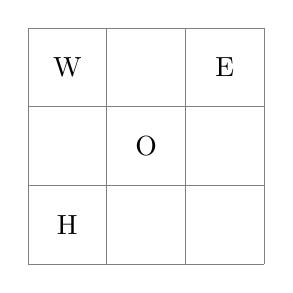
\begin{tikzpicture}
    \draw[step=1cm,gray,very thin,xshift=.5cm,yshift=.5cm] (-1,-1) grid (2,2);
    \node at (0cm,2cm) {W};
    \node at (0cm,0cm) {H};
    \node at (1cm,1cm) {O};
    \node at (2cm,2cm) {E};
  \end{tikzpicture}
  \caption{Example wumpus-world map.  W represents the initial
    location of the wumpus.  H represents the initial location of the
    human.  E represents the escape location.  O represents an
    obstacle that neither the human nor wumpus can move into.}
  \label{fig:map}
\end{figure}

\begin{quote}

\emph{\emph{Pursuit-evasion games} are scenarios with multiple agents
  where one agent attempts to avoid capture by another.  Consider a
  variation of pursuit-evasion games as follows:}

\begin{itemize}
  \item \it Two agents share a grid environment: a human (evader) and wumpus
  (pursuer).
  \item \it The human and wumpus alternate moves on the grid.  The
  wumpus moves each turn up, down, left or right.  The human can move
  up, down, left, right, or remain in place.  You may assume that the
  human moves first.
  \item \it If the wumpus and human ever occupy the same grid cell,
  the wumpus eats the human.
  \item \it If the human reaches a designated grid cell, they escape.
\end{itemize}

\emph{Answer the following questions using your implementation of finite
automata operations for support.}

\end{quote}

\begin{enumerate}

  \item For the map in \autoref{fig:map}, construct a discrete event
  system model.  Assume that the human's movements are controllable
  and that the wumpus's movements are not controllable.

  \item For your DES model of \autoref{fig:map}, construct a specification
  for the human to avoid the wumpus and escape.
  \begin{enumerate}
    \item Can the human guarantee to avoid being eaten, no matter what
    the wumpus does?  Prove yes or no via automata operations.
    \item Can the human always to escape in finite time (fixed
    number of steps), no matter what the wumpus does?  Prove yes or
    no.
  \end{enumerate}

  \item Design a map where the wumpus can always eat the human and
  prove via a DES model that this is the case.

  \item Design a map where the human can always escape and prove via a
  DES model that this is the case.

\end{enumerate}

\end{document}


%%% Local Variables:
%%% mode: latex
%%% TeX-master: t
%%% End:
